\documentclass[parskip=full,11pt]{scrartcl}
\usepackage[utf8]{inputenc}
\usepackage[T1]{fontenc}
\usepackage[german]{babel}
\usepackage[useregional]{datetime2}
\usepackage[pdfborderstyle={/S/U/W 0}]{hyperref}
\usepackage[nameinlink]{cleveref}
\usepackage[section]{placeins}
\usepackage{xcolor}
\usepackage{graphicx}
\usepackage{csquotes}
\usepackage{amsmath} % for $\text{}$
\usepackage{pflichtenheft}

\newcommand\urlpart[2]{$\underbrace{\text{\texttt{#1}}}{\text{#2}}$}

\crefname{figure}{Abb}{Abb}

\hypersetup{
	pdftitle={Pflichtenheft},
	bookmarks=true,
}

% section numbers in margins:
\renewcommand\sectionlinesformat[4]{\makebox[0pt][r]{#3}#4}

% header & footer
\usepackage{scrlayer-scrpage}
\lofoot{\today}
\refoot{\today}
\pagestyle{scrheadings}

\newcommand\producttitle{GO-App}

\title{Pflichtenheft: \producttitle}
\author{Lukas Dippon
        \and Jens Kienle
        \and Matthias Noll
        \and Fabian Röpke
        \and Tim Schmidt
        \and Simon Vögele}

\begin{document}
\maketitle

\section{Einleitung}
Studenten und Mitarbeiter des KIT treffen sich gerne zum gemeinsamen Essen oder Lernen.
Dazu ist an einem bestimmten Tag immer notwendig zu wissen, ob bereits ein Treffen vereinbart wurde.
Am Treffpunkt angekommen, möchte man wissen, an welchem Ort sich die Gruppe befindet, um nicht lange suchen zu müssen.
Unsere App soll es angemeldeten Benutzern ermöglichen, sich in Gruppen zu organisieren.
In den Gruppen kann der Zeit- und Treffpunkt bestimmt werden.
Nach der Festlegung des Treffens soll die App die GPS-Standorte der Mitglieder temporär und anonym anzeigen, um das Treffen zu vereinfachen.

\pagebreak
\section{Kriterien}
% Diese Section sollte kurz und knapp "für Manager" sein
% und auf eine Seite passen.

\subsection{Muss}
\criterium{Vereinfachte Treffpunkte}{crt:easy}{10}
Durch das Freigeben von Positionsdaten können andere Nutzer den
Standort bestimmen.

\criterium{Datenschutz}{crt:safe}{20}
Die Positionsdaten werden nur mit Bestätigung
des Nutzers gesendet und serverseitig nicht längerfristig gespeichert.

\criterium{Gruppen}{crt:groups}{30}
Mehrere Nutzer können sich in Gruppen zusammenschließen. In diesen
können sie Positionsdaten austauschen und Treffpunkte festlegen.
Ein Nutzer kann in beliebig vielen Gruppen Mitglied sein.

\criterium{1 zu 1 Verbindung}{crt:1to1}{40}
Die Position kann auf Wunsch auch mit nur mit einem anderen Nutzer geteilt werden

\criterium{Account}{crt:acc}{50}
Ein persönlicher Account ermöglicht es allen Nutzern,
Gruppenzugehörigkeiten und Datenschutzoptionen zu speichern.

\subsection{Kann}
\criteriumOptional{Abstimmungen}{crt:vote}{10}
Innerhalb von Gruppen können die Nutzer z.B. über nächste Treffpunkte abstimmen

\criteriumOptional{Detailliertere Innenraumkarten}{crt:indoor}{20}
Innenräume mit hoher Nutzerdichte bekommen detaillierte Innenraumkarten.

\criteriumOptional{Seite mit Betreiberinfo}{crt:about}{30}
Der Dienst bietet eine Seite \enquote{Über Uns},
mit Informationen zum Betreiber.

\subsection{Abgrenzung}
\criteriumNot{Keine Wahl Kurz-URL}{crt:no-choice}{10}
Ein Nutzer hat keine Möglichkeit die Auswahl einer Kurz-URL zu beeinflussen.

\pagebreak
%%%%%%%%%%%%%%
\section{Produkteinsatz}
Das Produkt dient zur Erleichterung des Zusammenfindens und der
Treffpunktvereinbarung in geschlossenen Gruppen von Freunden, Kollegen oder
Familienmitgliedern.

\subsection{Anwendungsbereiche}
\begin{itemize}
    \item Private Treffen in der Freizeit oder während der Arbeit
    \item Zusammenfindung auf größeren Veranstaltungen
\end{itemize}

\subsection{Zielgruppen}
\begin{itemize}
    \item Freundesgruppen
    \item Arbeitskollegen
\end{itemize}

\subsection{Betriebsbedingungen}
\begin{itemize}
    % TODO: Unschön formuliert
    \item Mobiler Einsatz in Umgebungen mit GPS-Empfang
\end{itemize}

%%%%%%%%%%%%%%
\section{Produktumgebung}
Das Produkt beinhaltet ein Client-Server-Modell.
Der Server dient lediglich als Vermittler zwischen Klienten.
Die Nutzer verwenden den Klienten auf ihrem mobilen Endgerät.
\subsection{Software}
\begin{itemize}
    \item Client: Android 4.1 (\enquote{Jelly Bean}, API-Level 16) oder
        höher.
    \item Server: Apache Tomcat 8
\end{itemize}

\subsection{Hardware}
% TODO: Mindestanforderungen an Hardware-Performance
\begin{itemize}
    \item Client: Android-fähiges mobiles Endgerät mit
        \begin{itemize}
            \item GPS-Empfänger
            \item Netzwerkkarte mit WLAN-Modul oder Mobilfunkeinheit
        \end{itemize}
    \item Server: Beliebiger Servercomputer, der Apache Tomcat 8 unterstützt
        und eine Internetanbindung besitzt
\end{itemize}

%%%%%%%%%%%
\section{Funktionale Anforderungen}

\functionality{Startmenü der App}{fnc:ui}{10}
unterteilt in 3 Tabs für die unterschiedlichen Funktionen
\begin{itemize}
    \item Liste aller Gruppen, in denen man Mitglied ist (\functionalitylink{fnc:groupfounding})
    \item Liste aller Events, an welchen man teilnimmt (\functionalitylink{fnc:eventlist})
    \item Liste aller Kontakte (\functionalitylink{fnc:1to1})
\end{itemize}

\functionality{Login in einen appspezifischen Account}{fnc:login}{20}
\fulfills{crt:acc}
Der Benutzer muss sich vor der Nutzung der App einen Account erstellen und sich mit diesem einloggen.

\functionality{Verwaltung von Einstellungen und Account- oder appbezogene Daten}{fnc:options}{30}
\fulfills{crt:acc}
Platzhalter % TODO: Beschreibung (siehe Bild mit Dragmenü)

\functionality{Gründen von Gruppen}{fnc:groupfounding}{40}
\fulfills{crt:groups}
Über einen Button am Listenende der Gruppenliste im Hauptmenü(\functionalitylink{fnc:ui}) können neue Gruppen
erstellt werden. Ihre Funktionen werden in \functionalitylink{fnc:groupmenu} bis \functionalitylink{fnc:votes}
beschrieben.

\functionality{Gruppenmenü}{fnc:groupmenu}{50}
\fulfills{crt:groups}
Jede Gruppe besitzt ein eigenes, in zwei Tabs eingeteiltes, Menü:
\begin{itemize}
		\item Chat(\functionalitylink{fnc:chat})
		\item Eventliste(\functionalitylink{fnc:groupevents})
\end{itemize}
Hier können ihre Funktionen angesteuert werden.

\functionality{Gruppenoptionen}{fnc:groupoptions}{60}
\fulfills{crt:groups}
Durch das Anklicken des Gruppennamen, öffnen sich die Gruppenoptionen. Hier können:
\begin{itemize}
		\item Mitglieder als Liste direkt eingesehen(\functionalitylink{fnc:memberlist})
		\item Mitglieder eingeladen oder entfernt(\functionalitylink{fnc:invitations})
		\item der Gruppenchat stumm geschalten %Anforderung fehlt
		\item Standortanfragen stumm geschalten %Anforderung fehlt
\end{itemize}
werden

\functionality{Liste der Gruppenmitglieder}{fnc:memberlist}{70}
\fulfills{crt:groups}
Es werden alle Mitglieder aufgelistet. Durch das Anklicken eines Mitgliedes kann wahlweise das
zugehörige Profil besucht oder das Mitglied aus der Gruppe entfernt werden.

\functionality{Einladen von Mitgliedern}{fnc:invitations}{80}
\fulfills{crt:groups}
Am Ende der Liste der Gruppenmitglieder(\functionalitylink{fnc:memberlist}) befindet sich ein Button,
um weitere Personen in die Gruppe einzuladen. Diese können von den eingeladenen Nutzern akzeptiert
oder abgelehnt werden.

\functionality{Eventliste}{fnc:groupevents}{90}
\fulfills{crt:groups}
\fulfills{crt:easy}
Jede Gruppe verfügt über eine Liste mit allen geplanten Events der Gruppe
(\functionalitylink{fnc:groupmenu})(\functionalitylink{fnc:events}).
Durch das Anklicken eines Events, öffnet sich eine Umgebungskarte, auf welcher der eigene Standort,
der Treffpunkt und alle freigegebene Standorte der Mitglieder markiert sind (\functionalitylink{fnc:locations}).

\functionality{Anfrage von GPS-Standorten}{fnc:locationrequest}{100}
\fulfills{crt:groups}
\fulfills{crt:easy}
\fulfills{crt:safe}
%% wie ist diese Funktion zu erreichen?
Erstellen einer GPS-Anfrage, bei der alle Gruppenmitglieder über ein Pop-Up gebeten werden, ihren Standort
für einen fest definierten Zeitraum freizugeben. Eine Standortanfrage erstellt ein temporäres Event ohne
spezifizierten Ort.

\functionality{Anzeigen von anonymen GPS-Standorten}{fnc:locations}{110}
\fulfills{crt:groups}
\fulfills{crt:easy}
\fulfills{crt:safe}
Alle GPS-Standorte der Grupenmitglieder, die aktuell freigestellt sind, werden erfasst und als Gruppierungen
auf der entsprechenden Karte(\functionalitylink{fnc:groupevents}) markiert. Diese Gruppierungen bestehen
aus geographisch nah beieinanderliegenden Gruppenmitgliedern. Einzelpersonen werden dabei unterscheidbar
von Gruppierungen symbolisiert.

\functionality{Events}{fnc:events}{120}
\fulfills{crt:groups}
Gruppenmitglieder können über einen Button in der Eventliste(\functionalitylink{fnc:groupevents}) ein neues Event,
bestehend aus Ort und einen Zeit, definieren. Das Event wird mit Uhrzeit in den
Eventlisten(\functionalitylink{fnc:eventlist})(\functionalitylink{fnc:groupevents}) aufgelistet.
Die Mitglieder werden eine kurze Zeit vor dem Event automatisch von der App durch ein Pop-Up gebeten,
ihren Standort für die entsprechende Umgebungskarte(\functionalitylink{fnc:groupevents}) temporär freizugeben.

\functionality{Gruppenchat}{fnc:chat}{130}
\fulfills{crt:groups}
Jede Gruppe verfügt über einen Chat (\functionalitylink{fnc:groupmenu}), in dem simple Nachrichten versandt
und Abstimmungen(\functionalitylink{fnc:vote}) erstellt werden können.

\functionality{Abstimmungen}{fnc:vote}{140}
\fulfills{crt:groups}
\fulfills{crt:vote}
Inerhalb des Gruppenchats(\functionalitylink{fnc:chat}) lassen sich Abstimmung erstellen. Diese werden bei
der Initialisierung vom Ersteller zeitlich begrenzt. Nach Erstellen der Abstimmung, wird diese als Event in den
Eventlisten(\functionalitylink{fnc:eventlist})(\functionalitylink{fnc:groupevents}) aufgelistet.
Inerhalb der Abstimmung lassen sich nun beliebig viele Treff- und Zeitpunkte hinzufügen,
sowie Stimmen abgeben und verändern. Alle, zur Wahl stehenden, Orte werden dabei als solche auf der zugehörigen
Karte (\functionalitylink{fnc:groupevents}) markiert. Nach Ablauf des Zeitlimits wird jeweils der Ort und die
Zeit mit den meisten Stimmen zum Zeit- bzw. Treffpunkt des Events und alle anderen Daten werden verworfen.
Hierbei wird bei einem Event ohne Ort, kein Ort auf der zugehörigen
Karte (\functionalitylink{fnc:groupevents}) markiert. Bei einem Event ohne final festgelegten Zeitpunkt
dagegen wird der aktuelle Zeitpunkt temporär oder ggf. final als Zeitpunkt des Events definiert.

\functionality{Standortteilung für einzelne Personen}{fnc:1to1}{150}
\fulfills{crt:1to1}
\fulfills{crt:easy}
\fulfills{crt:safe}
Es soll auch für Einzelpersonen möglich sein ihren Standort zu teilen.
Dies soll intern als Zweiergruppe implementiert sein, aber in der App als extra Reiter schnell
und ohne den Umweg über die Gruppengründung möglich sein.

\functionality{Eventliste}{fnc:eventlist}{160}
\fulfills{crt:groups}
In der Eventliste im Hauptmenü(\functionalitylink{fnc:ui}) werden alle Events aller Gruppen nach
Zeitpunkt sortiert angezeigt. Das Auswählen eines Events zeigt die entsprechende
Umgebungskarte(\functionalitylink{fnc:groupevents}) an.

%%%%%%%%%%%
\section{Nicht-Funktionale Anforderungen}

\nonFunctionality{Modernes Design}{nfc:design}{10}

Das Design soll modern und seriös wirken.

\nonFunctionality{Persistenz}{nfc:persistence}{20}

Sollten in Zukunft Erweiterungen oder Updates notwendig werden,
müssen die Daten (Kurz-URLs, E-Mailaddressen) erhalten bleiben.

\nonFunctionality{Erweiterbarkeit}{nfc:extensibility}{30}

Das Produkt muss dahingehend erweiterbar sein,
das die Liste der E-Mail-URL Abbildung von authentifizierten Nutzern
abgerufen werden kann.
Wie das genau implementiert wird, ist nicht Teil dieses Projekts.

%%%%%%%%%%%
\section{Tests}

\test{Gruppe Erstellen}{tst:grpcreate}{10}
\tests{fnc:login}

\teststep{Nutzer \enquote{Ned Stark} ist eingeloggt.}
{Ned tippt auf den Tab  \enquote{Gruppen}.}
{Er bekommt die Liste aller Gruppen angezeigt in denen er Mitglied ist.}

\teststep{Ned möchte eine Gruppe mit Leuten aus dem Fußball-Training erstellen.}
{Er tippt auf den \enquote{+}-Button (Neue Gruppe erstellen).}
{Er bekommt eine Liste all seiner Kontakte, die er im Produkt hinzugefügt hat, angezeigt.}

\teststep{Seine Freunde Robert B. und Edmund T. spielen ebenfalls Fußball.}
{Er tippt die beiden Namen an.}
{Das Produkt schlägt ihm vor die Gruppe zu erstellen.}

\teststep{Ned hat keine weiteren Freunde.}
{Er tippt auf Gruppe erstellen}
{Der Homescreen der Gruppe wird angezeigt.} % TODO: Homescreen?

%%%%%%%%%%%%%
\pagebreak
\appendix

\section{Seitenentwürfe}

% made via https://gomockingbird.com/projects/mnf0cwf/4gXVnC

\begin{figure}[hb]
	\fbox{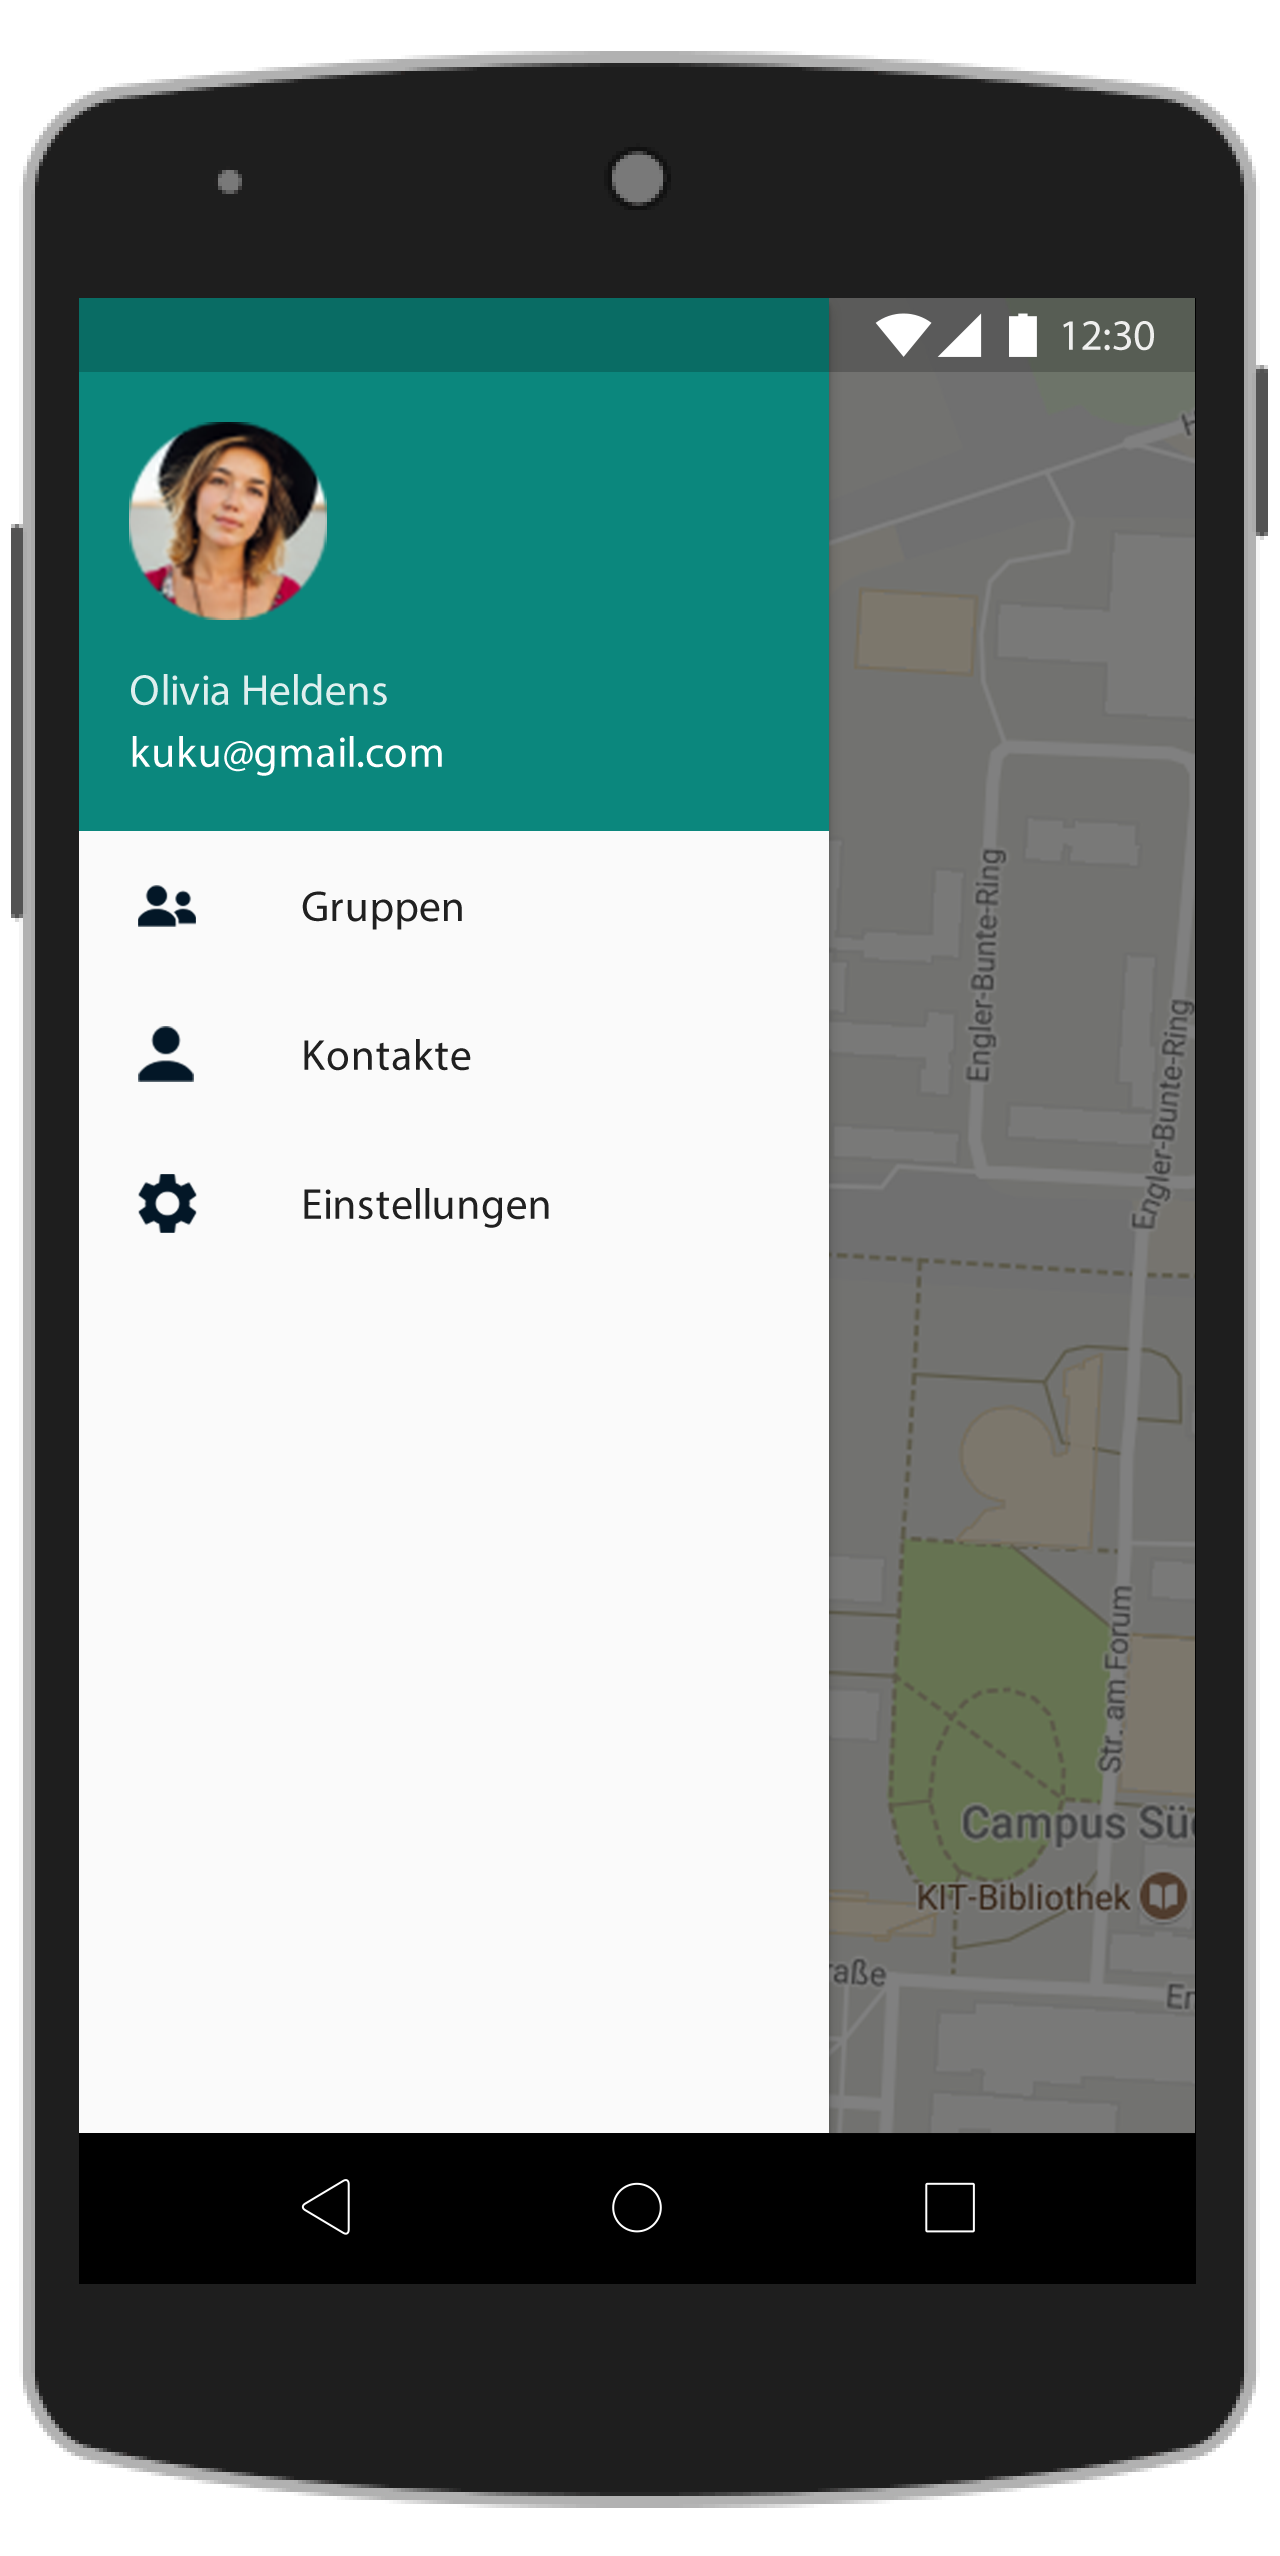
\includegraphics[height=80mm]{screenshots/menu.png}}
	\caption{\label{fig:menu}
		Menü mit der Möglichkeit auf Gruppen, Kontakte und Einstellungen zuzugreifen.
		 \testlink{tst:grpcreate}.
	}
\end{figure}

\begin{figure}[hb]
		\fbox{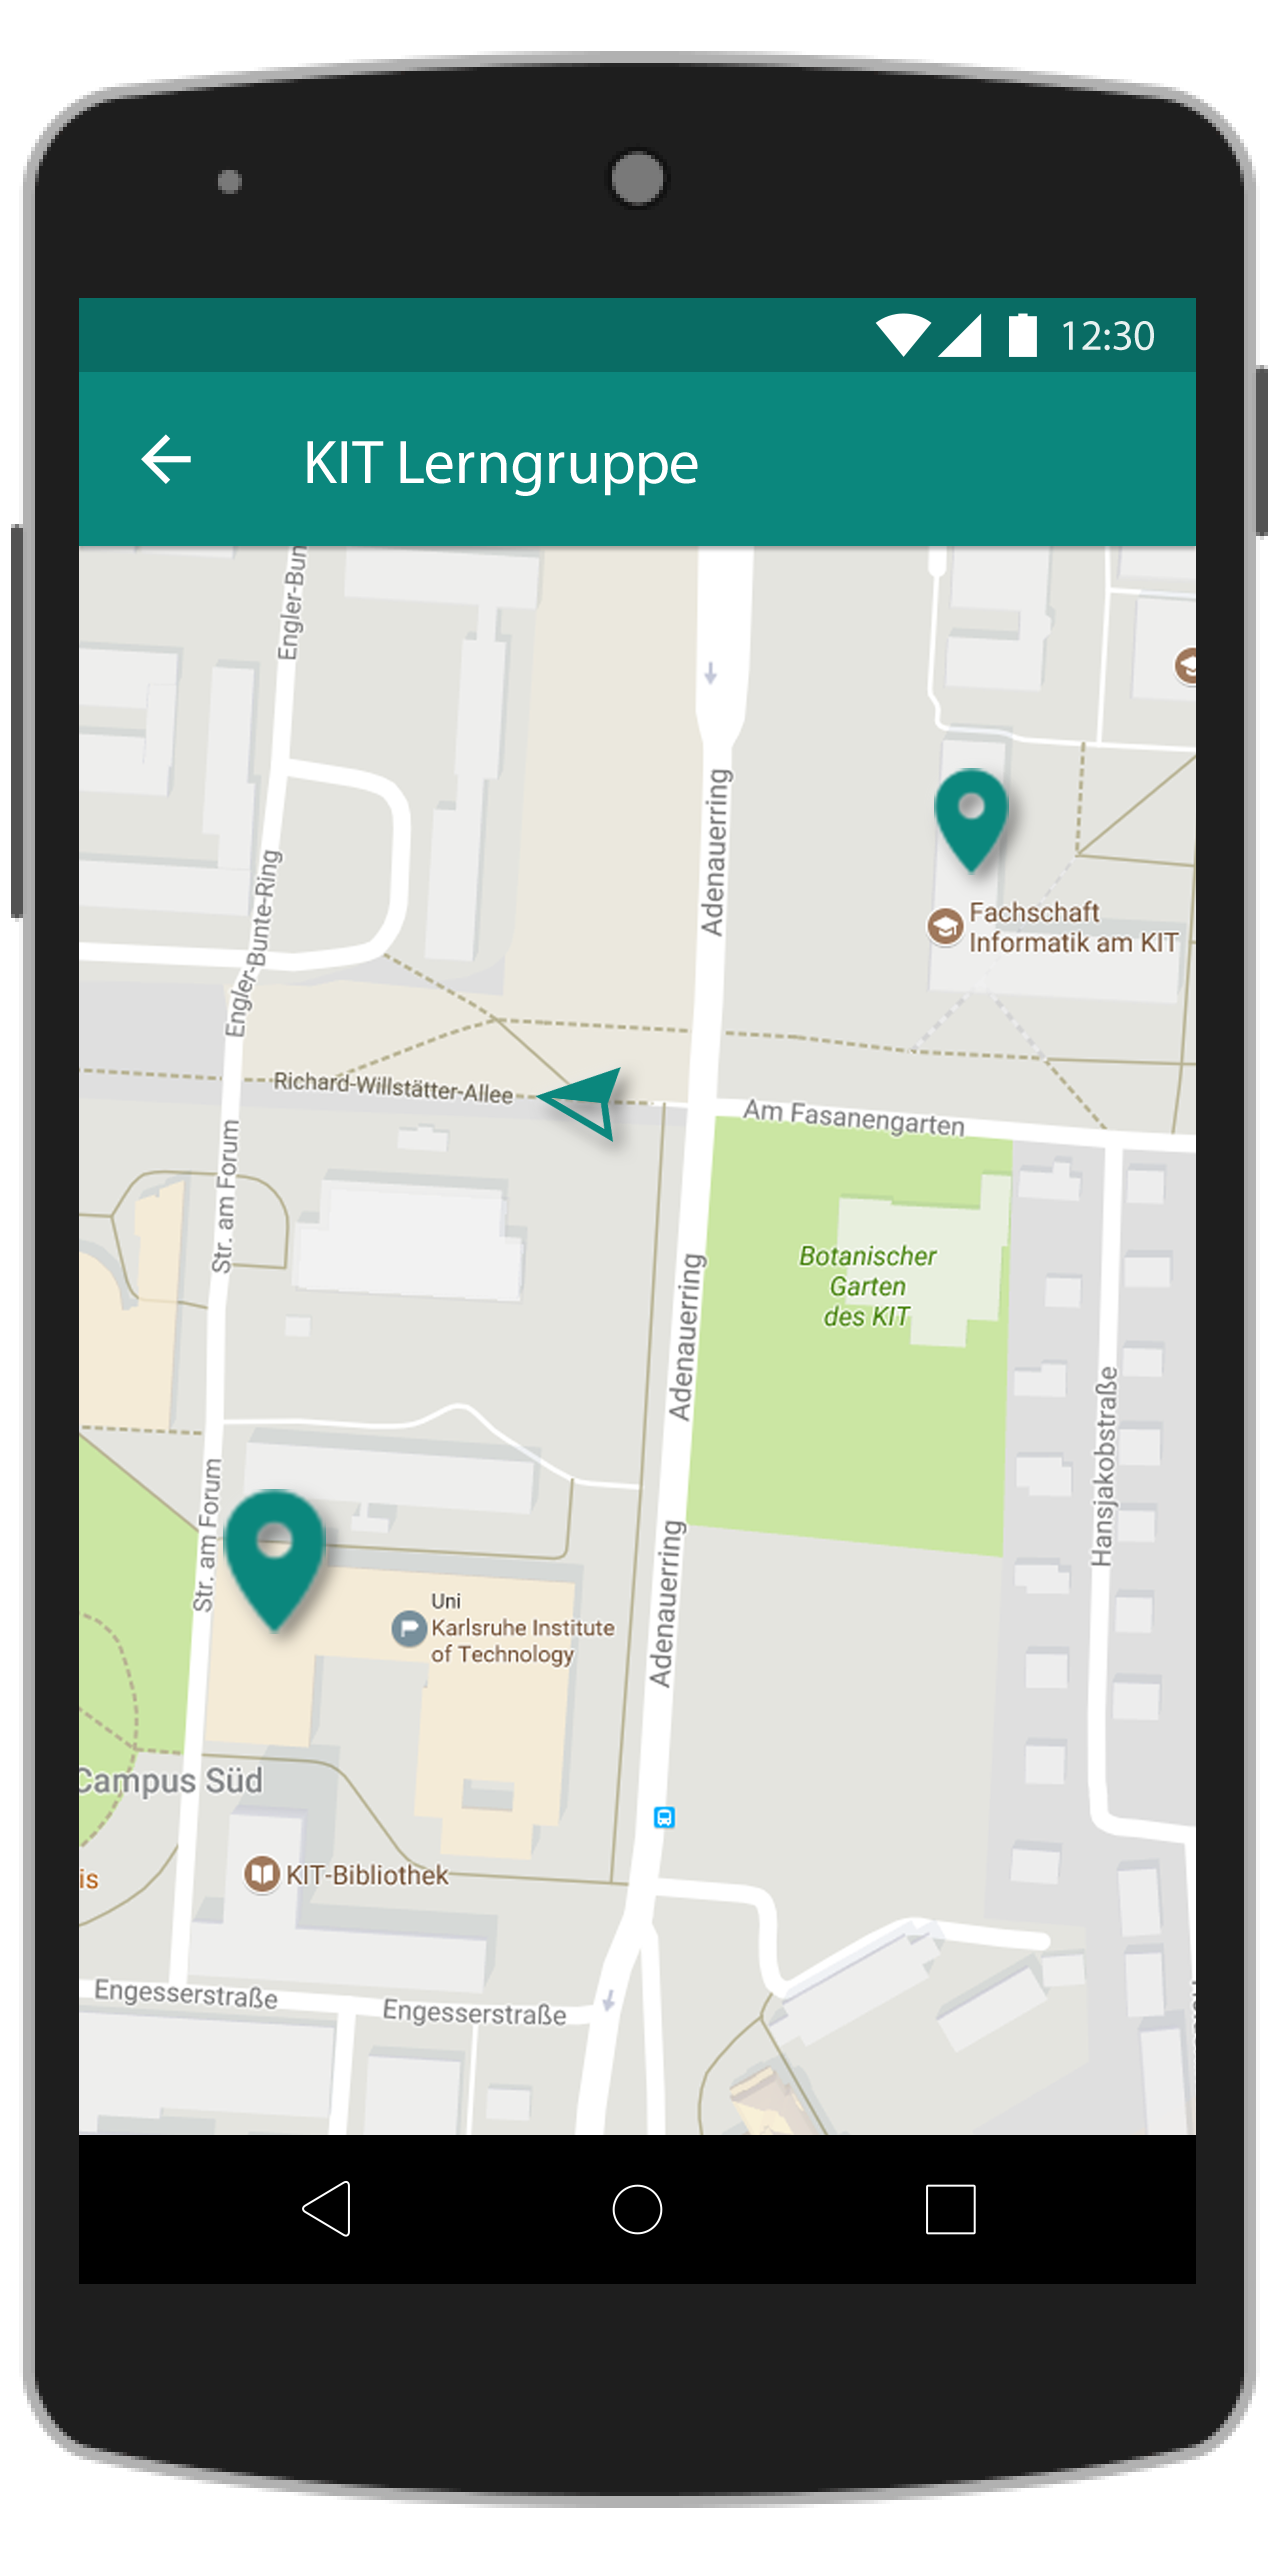
\includegraphics[height=80mm]{screenshots/karte.png}}
		\caption{\label{fig:map}
			Auf der Karte kann die Position der anderen Gruppenmitglieder eingesehen werden.
			Orte mit mehreren Mitgliedern erscheinen größer.
			\testlink{tst:grpcreate}.
		}
\end{figure}

\begin{figure}[hb]
		\fbox{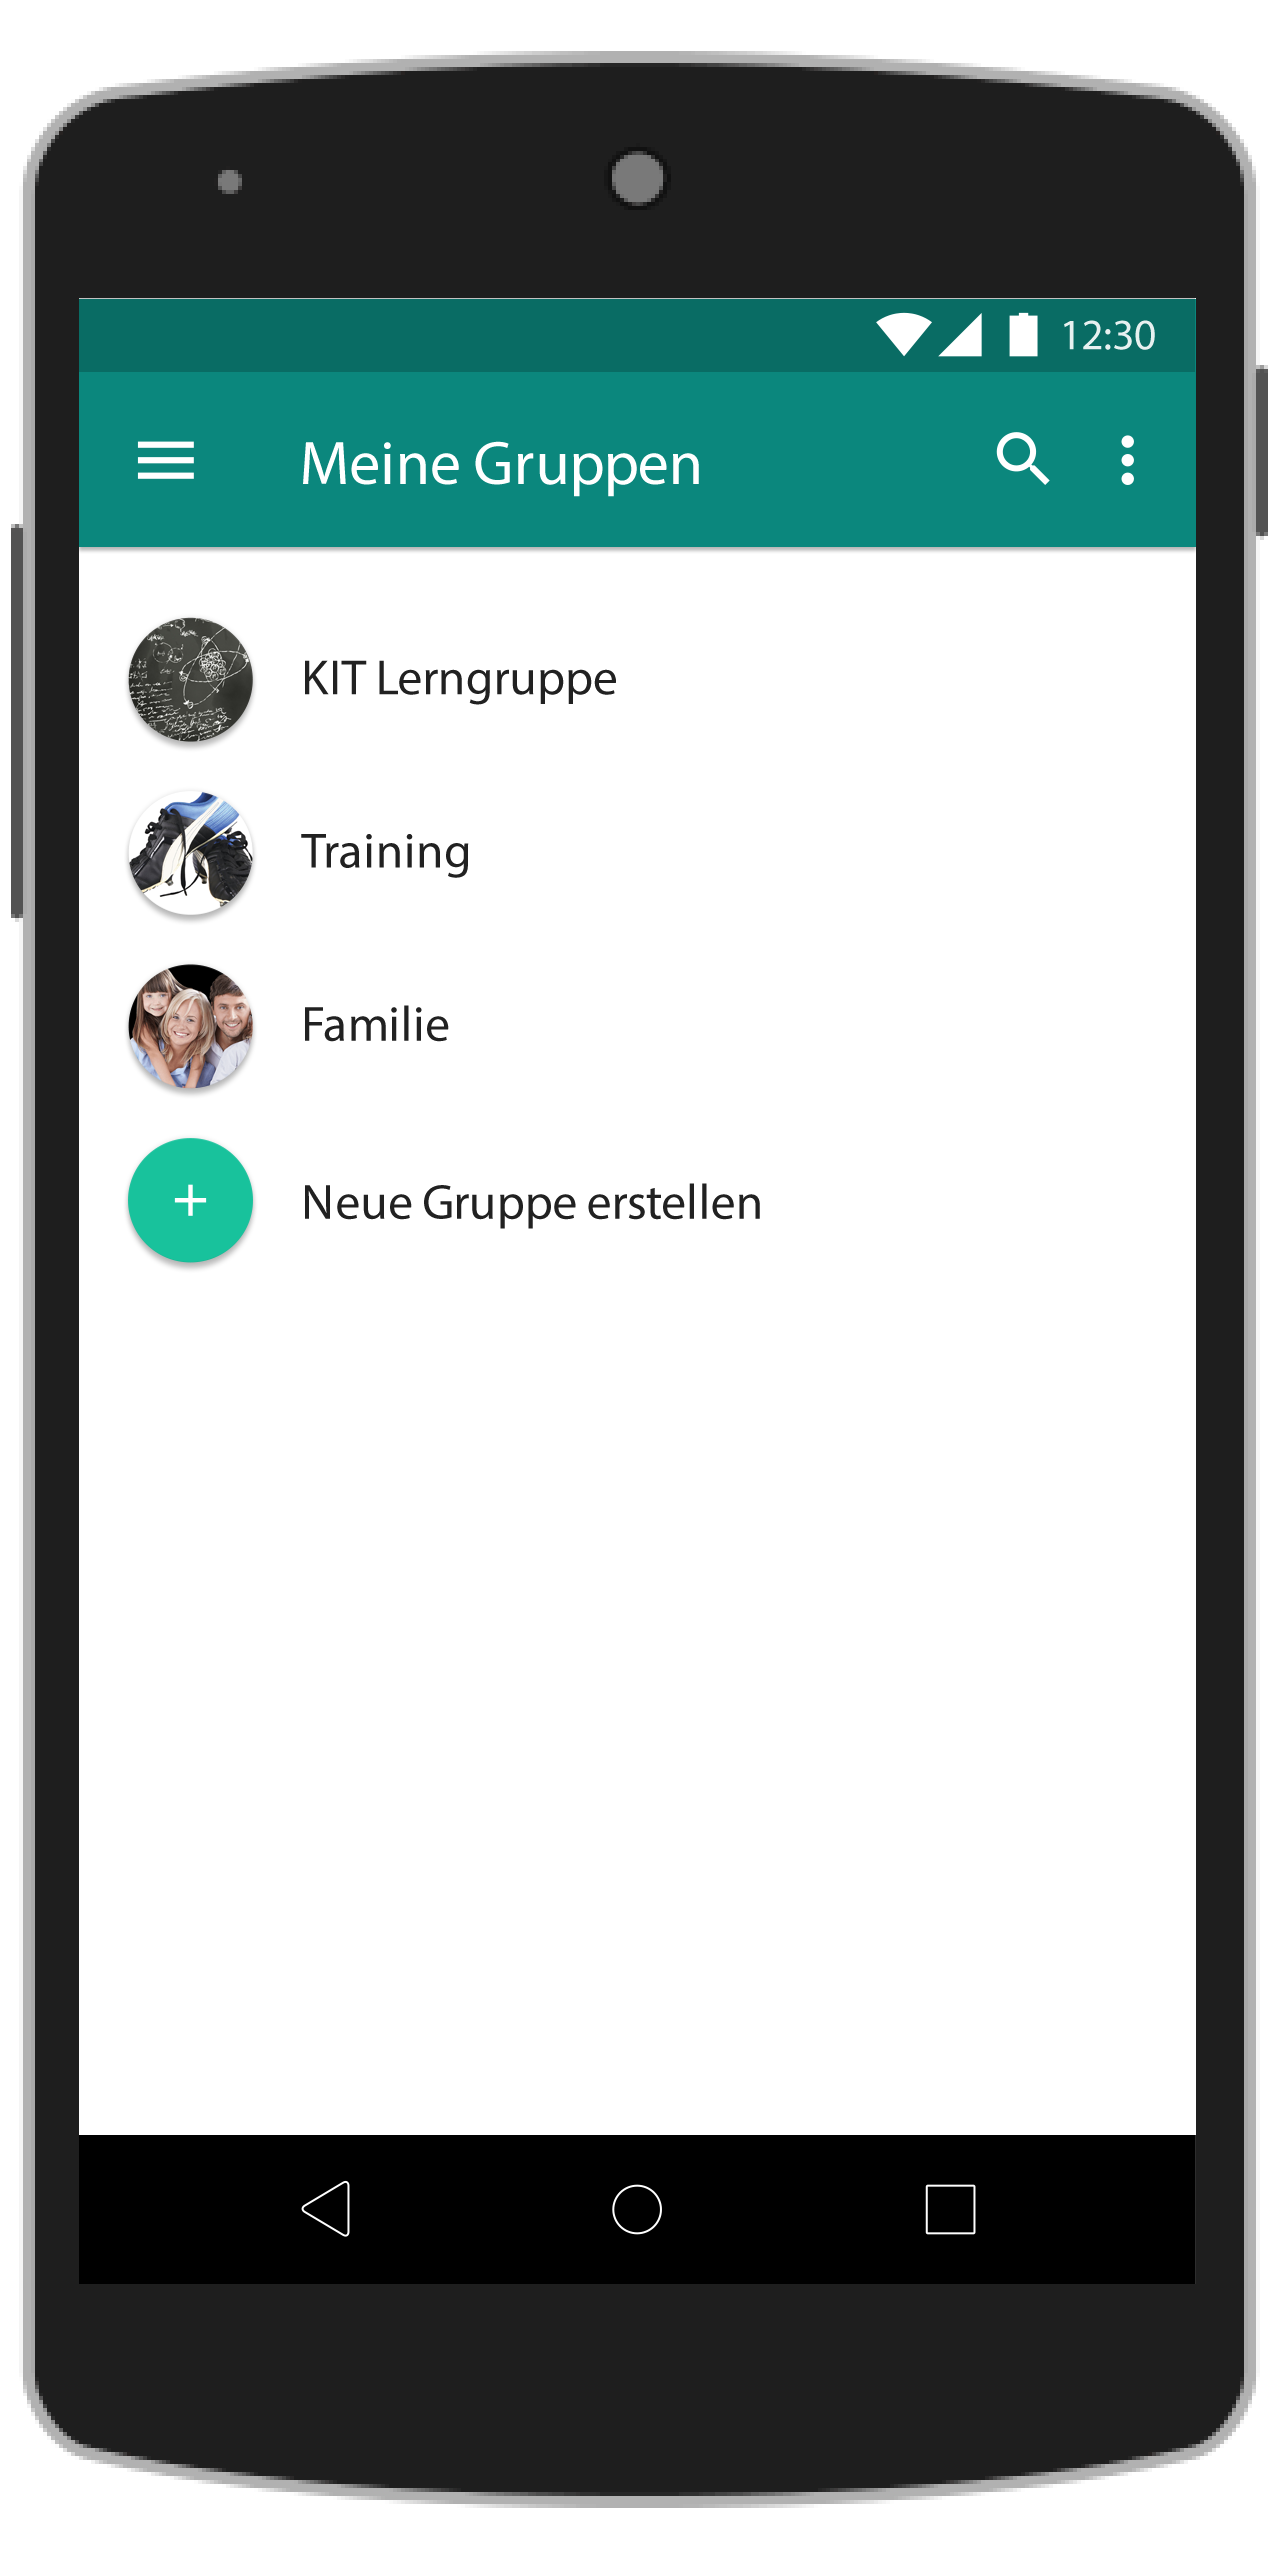
\includegraphics[height=80mm]{screenshots/gruppen.png}}
		\caption{\label{fig:groups}
			Hier können Gruppen verwaltet und angesehen, sowie neue hinzugefügt werden.
			\testlink{tst:grpcreate}.
		}
\end{figure}

\section{Glossar}

\textbf{Besucher}:
Eine Person, welche den Dienst nutzt.
Kann eingeloggt sein oder nicht.

\textbf{Dienst}:
Die Software im laufenden Betrieb. Software as a Service.

\textbf{Homepage}:
Seite, die beim Besuchen der Betreiberdomain \emph{ohne Pfad} angezeigt wird. Auch \enquote{Startseite}.

\textbf{Nutzer}:
Ein eingeloggter Besucher.

\end{document}
